%%%% Paramétrage du TD %%%%
\def\xxactivite{Activation 4 \ifprof -- Corrigé \else \fi} % \normalsize \vspace{-.4cm}
\def\xxauteur{\textsl{Xavier Pessoles}}

\def\xxnumchapitre{Chapitre 3 \vspace{.2cm}}
\def\xxchapitre{\hspace{.12cm} Application du Principe Fondamental de la Dynamique}

\def\xxtitreexo{Pendule}
\def\xxsourceexo{\hspace{.2cm} \footnotesize{Pendule}}
%\def\xxauteur{\textsl{Xavier Pessoles}}


\def\xxcompetences{%
\vspace{-.5cm}
\textsl{%
\textbf{Savoirs et compétences :}
\begin{itemize}[label=\ding{112},font=\color{ocre}] 
%\item \textit{Mod2.C16} : torseur cinétique
%\item \textit{Mod2.C17} : torseur dynamique
\item \textit{Mod2.C17.SF1} : déterminer le torseur dynamique d’un solide, ou d’un ensemble de solides, par rapport à un autre solide
%\item \textit{Mod2.C15} : matrice d'inertie
\item \textit{Res1.C2} : principe fondamental de la dynamique
\item \textit{Res1.C1.SF1} : proposer une démarche permettant la détermination de la loi de mouvement
%\item \textit{Res1.C2.SF1} : proposer une méthode permettant la détermination d’une inconnue de liaison
\end{itemize}
}}
\def\xxfigures{
%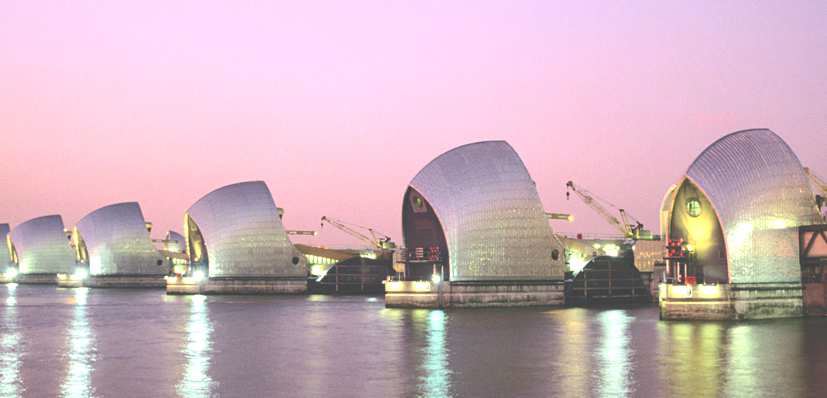
\includegraphics[width=.5\linewidth]{fig_00}
}%figues de la page de garde

\input{\repRel/Style/pagegarde_TD}
\setcounter{numques}{0}

\setlength{\columnseprule}{.1pt}

\pagestyle{fancy}
\thispagestyle{plain}

\ifprof
\vspace{5.1cm}
\else
\vspace{5.2cm}
\fi

\def\columnseprulecolor{\color{ocre}}
\setlength{\columnseprule}{0.4pt} 

%%%%%%%%%%%%%%%%%%%%%%%

\setcounter{exo}{0}



\ifprof
\else
\begin{multicols}{2}
\fi

\subsection*{Mise en situation}
On s'intéresse à un pendule guidé par une glissière. On fait l'hypothèse que le problème est plan. 

\begin{center}
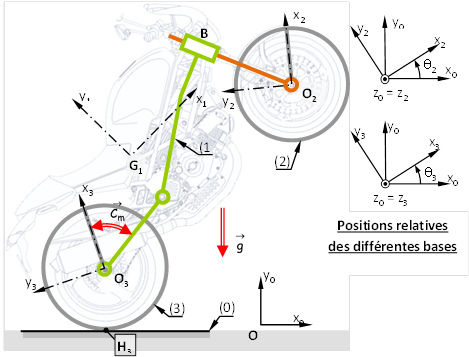
\includegraphics[width=.65\linewidth]{fig_01}
\end{center}
\begin{itemize}
\item On note 1 la pièce de masse $M_1$ et de centre de gravité $G_1$. $\vect{OA}=\lambda(t)\vect{x_0}-h\vect{y_0}$.
\item On note 2 la pièce de masse $M_2$ et de centre de gravité $G$ et de matrice d'inertie $\inertie{1}{G}= \matinertie{A}{B}{C}{-D}{-E}{-F}{\bas{2}}$. On a $\vect{AG}=L\vect{x_2}$
\end{itemize}

\subsection*{Travail à réaliser}

\question{Déterminer $\vectmd{A}{2}{0}$ en utilisant deux méthodes différentes. }
\ifprof
\begin{corrige}
~\\

\textbf{Cinématique}

On a $\vectv{G}{2}{0}=\derivvect{\vect{OG}}{\rep{0}} $ 
$=\derivvect{\lambda\vect{x_0}-h\vect{y_0}+L\vect{x_2}}{\rep{0}}$ 
$=\dot{\lambda}(t)\vect{x_0}+L\dot{\theta}\vect{y_2}$.



On a $\vectg{G}{2}{0}=\derivvect{\vectv{G}{2}{0}}{\rep{0}} $ 
$=\ddot{\lambda}(t)\vect{x_0}+L\ddot{\theta}\vect{y_2}-L\dot{\theta}^2\vect{x_2}$.

\textbf{Cinétique \& dynamique}


On a $\vectmd{G}{2}{0} = \derivvect{\vectmc{G}{2}{0}}{\rep{0}} $
\end{corrige}
\else
\fi



\question{En déduire le torseur dynamique $\torseurdyn{2}{0}$. }
\ifprof
\begin{corrige}
\end{corrige}
\else
\fi



\ifprof
\else
\end{multicols}
\fi

